\documentclass[10pt,a4paper]{article}
\usepackage[margin=0.56in,top=0.46in,bottom=0.48in]{geometry}
\usepackage[T1]{fontenc}
\usepackage{mathptmx,amsmath,amssymb,booktabs,graphicx,microtype,xcolor,hyperref}
\definecolor{ink}{HTML}{234C72}
\hypersetup{colorlinks=true,urlcolor=ink,citecolor=ink,linkcolor=ink}
\setlength{\parindent}{0pt}
\setlength{\parskip}{2.6pt}
\setlength{\columnsep}{0.25in}
\setlength{\emergencystretch}{1.5em}
\pagestyle{plain}
\newcommand{\sect}[1]{\vspace{4pt}{\color{ink}\fontsize{11}{12}\selectfont\bfseries #1}\par\vspace{1pt}}
\newcommand{\captext}[1]{{\footnotesize #1}\par}
\newcommand{\ind}{\mathbf{1}}
\begin{document}
\begin{center}
{\Large\bfseries SentinelRL: Budgeted Network Defence under Noisy Alerts}\par\vspace{4pt}
{\small\textbf{Rohit Mourya (B23ES1029)}\quad\textbf{Jyotiraditya Singh Rathore (B23ES1017)}}\par
{\small\href{https://github.com/rohitkumarmourya-maker/SentinelRL}{\texttt{github.com/rohitkumarmourya-maker/SentinelRL}}}\par\vspace{4pt}
{\small\color{ink}\textbf{FIXED-BUDGET STUDY --- THREE TRAINING SEEDS, 100 HELD-OUT SCENARIOS}}
\end{center}
\vspace{-2pt}
\small\textbf{Abstract.} SentinelRL allocates scarce defensive interventions in a synthetic network with stochastic compromise propagation and noisy alerts. A defender chooses inspection, patching, isolation, decoy deployment or waiting under a six-action budget. We formulate a finite-horizon partially observable Markov decision process (POMDP) and implement an observation-only Double DQN balancing critical-asset protection, detection delay and disruption. Across three independent agents and 100 paired test scenarios, Double DQN improves return over tabular Q-learning and random control, but shows no clear gain over an alert-based rule. Its low explicit-confirmation coverage reveals a containment--diagnosis trade-off.
\vspace{4pt}\hrule\vspace{4pt}

\begin{minipage}[t]{0.482\textwidth}\small
\sect{1. Practical problem and network}
A security operator cannot inspect or isolate every host immediately: false alarms consume analyst time, and unnecessary isolation disrupts legitimate services. The sequential question is which host to investigate or protect now while preserving resources for later threats. RL is appropriate because an action changes future exposure, observations and remaining budget; labels for an optimal action are unavailable.

The simulator contains six hosts and seven undirected reachability edges (Fig.~1). Vulnerabilities are $v=(.40,.68,.58,.82,.76,.48)$ and criticalities are $c=(.45,.62,.80,1.00,.52,.96)$ for hosts $0$--$5$. A host is critical when $c_i\geq .80$. Each episode lasts $T=48$ steps and starts with budget $B_0=6$. One hidden foothold is sampled at host $0$ with probability $.62$, otherwise host $4$; its identity is not given to the defender.

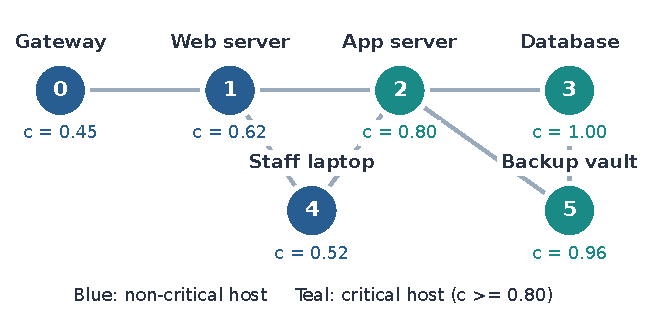
\includegraphics[width=\linewidth]{assets/topology.pdf}
\captext{\textbf{Fig. 1.} Fixed simulated network; labels show criticality. Edges represent possible lateral movement, not observed infections.}

\sect{2. Hidden state and observations}
The POMDP is $(\mathcal S,\mathcal A,P,\mathcal O,\Omega,R,\gamma)$~\cite{pomdp}. Its complete reward-relevant state has \textbf{56 dynamic components}: per host, compromise $z$, patch $p$, isolation $\ell$, decoy $d$, alert, EWMA, last inspection result, last inspection time and ever-confirmed flag (54), plus budget $B_t$ and time $t$. The physical flags alone are 24 bits. Graph, $v$ and $c$ are fixed constants. Compromise and the ever-confirmed flags are omitted from the policy input; historical results may become stale.

The policy input is $o_t\in[0,1]^{56}$: \textbf{nine features per host} (54) plus $B_t/6$ and $t/48$. Host features are current alert, alert exponentially weighted moving average (EWMA), last explicit inspection result, normalized inspection age, $v_i,c_i,p_{t,i},\ell_{t,i},d_{t,i}$. Inspection results encode unknown/clean/compromised as $0/.5/1$; unknown inspection age is $1$. EWMA uses weight $.35$ for the current alert. A past clean result remains stale if a hidden infection occurs later. The observation is a compact history summary, not an exact sufficient belief state. True infection counts and entry identity are excluded.
\end{minipage}\hfill
\begin{minipage}[t]{0.482\textwidth}\small
\sect{3. Stochastic dynamics and actions}
After the selected action, time advances and every previously compromised, non-isolated source can infect each susceptible non-isolated neighbour $j$ with probability
\begin{equation*}
P(i\!\rightarrow\!j)=.23\,v_j\,(.20)^{p_{t,j}}(.25)^{d_{t,j}}.
\end{equation*}
Spread is simultaneous: a newly infected host first spreads on the next step. Isolation blocks both incoming and outgoing movement. Patching and decoys reduce future infection risk; neither cures an existing infection. Independent pre-sampled edge/time random numbers support reproducible comparisons. There is no adaptive attacker or real network traffic.

Non-isolated hosts emit binary alerts with
\begin{equation*}
\begin{aligned}
P(y_{t,i}=1\mid z_{t,i}=1)&=.55,\\
P(y_{t,i}=1\mid z_{t,i}=0)&=.08.
\end{aligned}
\end{equation*}
The initial observation also comes from this sensor. Alerts update EWMA and are not ground-truth confirmations.

\textbf{Action space.} $\mathcal A=\{0,\ldots,24\}$ contains \texttt{WAIT} and four host-specific actions: six each of \texttt{INSPECT}, \texttt{PATCH}, \texttt{ISOLATE}, \texttt{DECOY}. Each valid intervention spends one token; \texttt{WAIT} spends none. Inspection reveals the current state of that host. A mask derived solely from observable deployment flags, time and budget prevents unavailable actions; waiting is always legal. This legality mask does not enforce a favourable policy or consult hidden compromise.

\sect{4. Reward and incentive design}
Let $u_t$ mark a valid non-wait action, $q_t$ an invalid action, $f_t$ a first-ever successful explicit confirmation, $N_t$ newly compromised hosts, $U_t$ unisolated compromised hosts after spreading, and $F_t$ a clean host newly isolated by this action. Let $L_t$ be all clean isolated hosts, $H_t$ active hosts never explicitly confirmed, and $K_t=\{j\in U_t:c_j\geq .80\}$. The scalar reward is
\begin{align*}
r_t={}&-.16u_t-.45q_t+.40f_t\\
 &-\sum_{j\in N_t}(2+4c_j)-.16\sum_{j\in U_t}c_j\\
 &-\sum_{j\in F_t}(.65+.85c_j)-.03\sum_{j\in L_t}c_j\\
 &-.04\sum_{j\in H_t}c_j-1.4\ind[t=T]\,|K_t|.
\end{align*}
The objective is $\max_\pi\mathbb E_\pi[\sum_{t=1}^{T}\gamma^{t-1}r_t]$. New compromises incur larger losses on valuable assets; active compromise incurs ongoing damage, with an extra penalty until explicit confirmation. False isolation has immediate and persistent service costs. A one-time confirmation bonus values information without rewarding repeated inspection of the same infection. Patch, decoy and correct isolation earn no direct positive bonus: their value comes from avoided future losses. Hidden state is used by the simulator to calculate reward and evaluation metrics, not by the deployed policy input.
\end{minipage}

\newpage
\begin{minipage}[t]{0.482\textwidth}\small
\sect{5. Algorithm and completed training}
DQN~\cite{dqn} learns action values from replayed transitions and a target network. Double DQN~\cite{ddqn} separates action selection from evaluation to address maximization bias. A two-layer ReLU MLP (128 units each) maps 56 observed features to 25 values. Exploration is $\epsilon$-greedy over legal actions; masks also constrain the bootstrap target. For terminal flag $d$ and next legal-action mask $m'$,
\begin{align*}
a^*&=\arg\max_{a':m'(a')=1}Q_\theta(o',a'),\\
y&=r+\gamma(1-d)Q_{\bar\theta}(o',a^*),\\
\mathcal L(\theta)&=\mathbb E[\operatorname{Huber}(Q_\theta(o,a)-y)].
\end{align*}
We use $\gamma=.98$, Adam $3\times10^{-4}$, batch 64, replay 50,000, warm-up 1,000 steps, one update per four steps, target synchronization every 500 updates and gradient-norm clipping at 10. Exploration falls from $1$ to $.05$ over 80,000 steps. Each seed ($17,29,43$) completes 2,500 episodes, 120,000 transitions and 29,751 gradient updates on CPU, with verified parameter changes. Checkpoints are the fixed final iterates, without test-based selection.

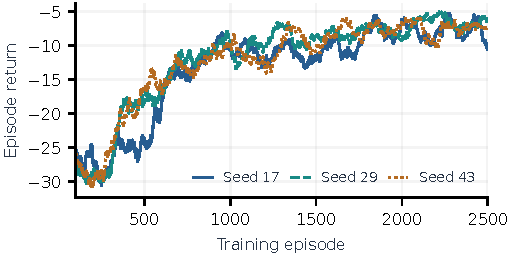
\includegraphics[width=\linewidth]{assets/training_measured.pdf}
\captext{\textbf{Fig. 2.} Actual $\epsilon$-greedy training return: 100-episode moving means for three independent seeds. These descriptive curves have no confidence bands and differ from greedy held-out evaluation.}

\sect{6. Primary results and ablations}
On the prespecified held-out set (Fig.~3), DDQN return is $-10.04$ (95\% CI $[-13.60,-6.87]$), with seed means $-10.58,-11.03,-8.52$ (SD $1.34$). Paired return gains are $21.83$ over tabular Q-learning (CI $[15.77,27.95]$), $15.91$ over random control ($[9.57,22.16]$), and $33.06$ over initialization ($[26.59,39.99]$).

The alert rule is stronger than those baselines: its return is $-9.48$, and DDQN minus rule is $-0.56$ (CI $[-4.70,3.25]$). This does not establish superiority or equivalence. Retraining without EWMA and inspection history gives return $-14.12$; the full model's paired gain is $4.08$ ($[.99,7.84]$), with $.21$ fewer critical compromises ($[-.43,-.02]$ for full minus ablated). These exploratory intervals rely on only three training seeds.

\textbf{Diagnostic weakness.} DDQN confirms only $2.64\%$ of infected hosts per episode on average, versus $91.13\%$ for the alert rule (Table~1). Mean censored confirmation delay is $45.40$ versus $5.05$ steps. Isolation can contain an attacker without explicit inspection; an isolated but unconfirmed infection still contributes a censored delay. Thus return/containment gains do not imply successful diagnosis, and this controller does not satisfy every defence objective.
\end{minipage}\hfill
\begin{minipage}[t]{0.482\textwidth}\small
\sect{7. Evaluation design and limitations}
Training environment seeds are $10^6s+i$ for training seed $s$ and episode index $i$. Greedy evaluation uses 100 unseen scenarios, $300000+97i$, $i=0,\ldots,99$, shared across policies through pre-sampled noise. No hyperparameters or checkpoints were selected on these outcomes. Tabular Q-learning receives the same training budget. A retrained no-memory DDQN removes EWMA, inspection result and inspection age; the untrained control uses the initial weights. Alert-rule, random-legal and wait-only policies provide operational controls.

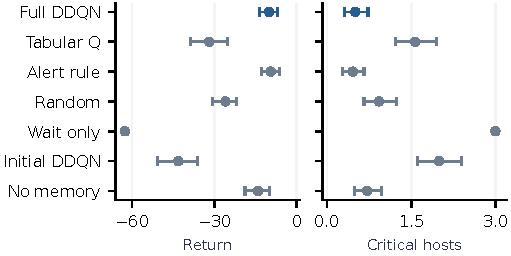
\includegraphics[width=\linewidth]{assets/comparison_measured.pdf}
\captext{\textbf{Fig. 3.} Primary held-out means and 95\% crossed-bootstrap intervals: three seed blocks and 100 shared scenarios, 2,000 resamples of seed rows and paired scenario columns. Higher return and fewer critical hosts are preferable. Fixed rules are deterministic across seed blocks; repeated copies add no independent scenarios.}

\begin{center}\footnotesize
\setlength{\tabcolsep}{4pt}
\begin{tabular}{lrrrr}
\toprule
\textbf{Policy} & $U$ & $F$ & $C\%$ & $D$\\
\midrule
DDQN & .713 & .280 & 2.64 & 45.40\\
Alert rule & .580 & .000 & 91.13 & 5.05\\
Tabular Q & 3.230 & .187 & 13.79 & 34.19\\
Random & 2.470 & 1.260 & 12.35 & 36.33\\
Wait only & 5.990 & .000 & .00 & 38.15\\
\bottomrule
\end{tabular}
\end{center}
\captext{\textbf{Table 1.} Primary held-out means. $U$: uncontained hosts at $T$; $F$: clean-host isolations (both hosts/episode); $C$: mean within-episode fraction of infected hosts explicitly confirmed; $D$: censored confirmation delay (steps). Intervals and per-seed values for all metrics are in the raw result tables.}

For infected host $i$, delay is $\min(t_i^{\rm confirm},T)-t_i^{\rm infection}$, setting $t_i^{\rm confirm}=\infty$ if unconfirmed. We average within episode before averaging episodes. Censoring and infection timing prevent treating this measure alone as true detection latency; confirmation coverage must accompany it. Critical compromises count hosts ever infected, not incidents contained.

\textbf{Sensor sensitivity.} An independent 100-scenario set ($400000+97i$), paired across sensor conditions without retraining, gives DDQN returns $-13.30,-7.16,-3.80$ at detection sensitivities $.35,.55,.75$; rule returns are $-20.17,-12.97,-9.15$. False-positive rate remains $.08$. This auxiliary set does not replace the primary comparison; its different base-condition outcome illustrates scenario-sample uncertainty.

\textbf{Scope.} The fixed synthetic topology, calibrated costs, stationary attacks and simplified service impact limit external validity. The observation is compressed history, not a sufficient belief state. With three training seeds, uncertainty estimates remain exploratory. The repository includes trained checkpoints, raw episode/update logs, manifests and reproduction commands. All 35 tests pass. Logged CPU training time for the three main DDQN runs totals 45.0\,s on an Apple M5 Max CPU with one Torch thread (excluding evaluation). No real-network effectiveness is claimed.
\vspace{2pt}
{\footnotesize
\begin{thebibliography}{3}
\setlength{\itemsep}{1pt}\setlength{\parskip}{0pt}
\bibitem{pomdp} L.~P.~Kaelbling, M.~L.~Littman and A.~R.~Cassandra. Planning and acting in partially observable stochastic domains. \emph{Artificial Intelligence} 101:99--134, 1998. \href{https://people.csail.mit.edu/lpk/papers/aij98-pomdp.pdf}{Author full text}.
\bibitem{dqn} V.~Mnih et al. Human-level control through deep reinforcement learning. \emph{Nature} 518:529--533, 2015. \href{https://doi.org/10.1038/nature14236}{doi:10.1038/nature14236}.
\bibitem{ddqn} H.~van Hasselt, A.~Guez and D.~Silver. Deep reinforcement learning with Double Q-learning. \emph{AAAI}, 2016. \href{https://arxiv.org/abs/1509.06461}{arXiv:1509.06461}.
\end{thebibliography}}
\end{minipage}
\end{document}
